\documentclass[compress, notes=hide]{beamer}
%\documentclass[compress, notes=hide,handout]{beamer}

\usepackage[T1]{fontenc}
\usepackage{lmodern}
\usepackage{textcomp}
\graphicspath{{../figures/}}
\usepackage[english,norsk]{babel} %norske navn rundt omkring

\usepackage[latin1]{inputenc} %Norsk tegnsetting
\usepackage{amsmath,amsfonts,amssymb,mathrsfs} %matematikksymboler
\usepackage{algorithm, algorithmic}
\usepackage{amsthm} %for � lage teoremer og lignende.
\usepackage{bm} %fikser bold math-problematikken
%\usepackage[hang]{subfigure} %hvis du vil kunne ha flere figurer inni en figur
%\usepackage[small,bf,hang]{caption} %bestemmer format p� figurtekst
\usepackage{multirow}
\usepackage{graphpap}
\usepackage{pgf} %Tegning
\def\pgfex{ex}
%\usepackage{mathptmx}
%\usepackage{helvet}
%\usepackage{verbatim}

\setbeamertemplate{caption}[]
\setbeamertemplate{navigation symbols}{}
%\setbeamertemplate{footline}[page number]
\setbeamertemplate{footline}[frame number]
%\setbeamertemplate{caption}[numbered] 
\usecolortheme{default}
%\usetheme{Pittsburgh} %\usetheme{Singapore}
\setbeamertemplate{itemize item}[circle] %triangel p� 2-level-itemize (for 1-level brukt {itemize item})
\setbeamertemplate{itemize subitem}[triangle] %triangel p� 2-level-itemize (for 1-level brukt {itemize item})
\setbeamertemplate{section in toc}[circle]{} %Nummer i table of content
\setbeamertemplate{enumerate items}[circle] 
\setbeamertemplate{itemize subitem}[triangle] %triangel p� 2-level-itemize (for 1-level brukt {itemize item})
\setbeamercolor{itemize subitem}{fg=gray} %farge bullets

% For � skrive i default bl� farge:
% \textcolor[rgb]{0.2,0.2,0.7}{Blablabla-tekst}
%\newcommand{\hl}[1]{\textcolor[rgb]{0.2,0.2,0.7}{\emph{#1}}}
\newcommand{\hl}[1]{\textbf{#1}}
\newcommand{\hlb}[1]{\textcolor[rgb]{0.2,0.2,0.7}{#1}}
\newcommand{\sectionheader}{
    \usebeamerfont*{section number projected}%
    \usebeamercolor{section number projected}%
    \begin{pgfpicture}{-1ex}{-0.4ex}{1ex}{2ex}
      \color{bg}
      \pgfpathcircle{\pgfpoint{0pt}{.75ex}}{1.2ex}
      \pgfusepath{fill}
      \pgftext[base]{\color{fg}\thesection}
    \end{pgfpicture}\kern1.25ex
   \usebeamercolor[bg]{item projected}
    \Large{\insertsectionhead}
}

% FOR Å SKRIVE I DEFAULT, BLÅ FARGE:       \textcolor[rgb]{0.2,0.2,0.7}{Blablabla-tekst}

\title{Analysis of contingency tables}
\subtitle{Chi-squared and (Fisher's) exact tests}
\author{Chi Zhang\\
\footnotesize{Oslo Center for Biostatistics and Epidemiology}\\
\footnotesize{Department of Biostatistics, UiO}\\
\footnotesize{chi.zhang@medisin.uio.no}}
\date{MF9130 -- Introductory Course in Statistics\\
02.02.2023}


\setbeamertemplate{navigation symbols}{}
%\setbeamertemplate{footline}[page number]
\setbeamertemplate{footline}[frame number]
\usecolortheme{default}
%\setbeamertemplate{background}[grid][step=0.25cm]%Rutenett

\begin{document}

\section{Title page}

\frame{\titlepage}

\section{Overview}

\section{Overview}

\frame{ 
\frametitle{Overview}
  \begin{block}{Aalen chapter 6.5, Kirkwood and Sterne chapter 17}
    \begin{itemize}
    \item Chi-squared tests for 2x2 contingency tables
     \textcolor{red}{20}
    \item Exact tests  \textcolor{red}{10min}
    \item Larger contingency tables \textcolor{red}{plus remarks. 20min}
    \item STATA for table analysis \textcolor{red}{20m}
    \end{itemize}
  \end{block}
}

\frame{ 
  \frametitle{}
  \begin{block}{Last lecture}
    \begin{itemize}
    \item Proportions for one group, tests
    \item Proportions for two groups, three measures (RD, RR, OR)
    \end{itemize}
  \end{block}
  \begin{block}{This lecture}
    \begin{itemize}
    \item \textbf{Chi-squared test}
    \item \textbf{Fisher's exact test}
    \item How to implement in STATA
    \end{itemize}
  \end{block}
}


\frame{ 
	\frametitle{Chi-squared test for $2 \times 2$ table}
	\textbf{Pearson's chi-squared test} (test of independence): whether the observations that measure two variables are independent of each other, i.e. no association.
	
	\begin{block}{}
		 The \hl{test statistic} is
		\begin{equation}
		 	\chi^2 = \sum_i \frac{(O_i-E_i)^2}{E_i}, \quad \mathrm{d.f.} = 1,\nonumber
		 \end{equation}
		 where $O_i$ and $E_i$ denote the \textbf{observed} and\textbf{ expected} values in the
		 $i$th cell
		 
	\vspace{0.2cm}
	For a $2 \times 2$ table, under the null hypothesis (of no association between the two variables), the test statistic is \textbf{chi-squared distributed with 1 degree of freedom}.
	\end{block}

\textcolor{red}{first look at an example, then explain the logic (e.g. what does df mean, what does expected mean)}
}



% example 17.1 -----

\begin{frame}
	\begin{block}{Example 17.1 in Kirkwood \& Sterne}
		We consider data from an \hl{influenza vaccination trial}. In this case the exposure is vaccination (the row variable), so the table includes row percentages.
		\begin{table}
			\begin{small}
				\begin{tabular}{lccc}
					\textbf{Observed numbers} & & &
					\\
					\hline
					& \multicolumn{2}{c}{\textbf{Influenza}} &
					\\
					\cline{2-3}
					& \textbf{Yes} & \textbf{No} & \textbf{Total}
					\\
					\hline
					\textbf{Vaccine} & 20 (8.3\%) & 220 (91.7\%) & 240
					\\
					\textbf{Placebo} & 80 (36.4\%) & 140 (63.6\%) & 220
					\\
					\hline
					\textbf{Total} & 100 (21.7\%) & 360 (78.3\%) & 460
					\\
					\hline
				\end{tabular}
			\end{small}
		\end{table}
		We want to assess the strength of the evidence that vaccination
		affected the probability of getting influenza.
	\end{block}
\end{frame}



\begin{frame}
	\begin{block}{}
		We start by calculating the \hl{expected numbers} \textit{under the
		assumption of no association} between vaccination and subsequent
		contraction of influenza. \textcolor{red}{explain no association}
		
		\vspace{0.2cm}
		Overall 100/460 (21.7\%) people got influenza, so the expected numbers
		\hl{getting influenza} are:
		\begin{itemize}
			\item{$100/460 \times 240 = 52.2$ in the vaccine group, and}
			\item{$100/460 \times 220 = 47.8$ in the placebo group.}
		\end{itemize}
		Further, overall 360/460 (78.3\%) people escaped influenza, so the expected numbers \hl{escaping influenza} are:
		\begin{itemize}
			\item{$360/460 \times 240 = 187.8$ in the vaccine group, and}
			\item{$360/460 \times 220 = 172.2$ in the placebo group.}
		\end{itemize}
	\end{block}
\end{frame}


\begin{frame}
	\begin{block}{Observed numbers}
				\begin{table}
			\begin{small}
				\begin{tabular}{lccc}
					\hline
					& \multicolumn{2}{c}{\textbf{Influenza}} &
					\\
					\cline{2-3}
					& \textbf{Yes} & \textbf{No} & \textbf{Total}
					\\
					\hline
					\textbf{Vaccine} & 20 (8.3\%) & 220 (91.7\%) & 240
					\\
					\textbf{Placebo} & 80 (36.4\%) & 140 (63.6\%) & 220
					\\
					\hline
					\textbf{Total} & 100 (21.7\%) & 360 (78.3\%) & 460
					\\
					\hline
				\end{tabular}
			\end{small}
		\end{table}
		
	\end{block}
	\begin{block}{Expected (assume independence between vaccine and influenza)}
	\begin{table}
		\begin{small}
			\begin{tabular}{lccc}
				\hline
				& \multicolumn{2}{c}{\textbf{Influenza}} &
				\\
				\cline{2-3}
				& \textbf{Yes} & \textbf{No} & \textbf{Total}
				\\
				\hline
				\textbf{Vaccine} & \textcolor{blue}{52.2} (21.7\%) & \textcolor{blue}{187.8} (78.3\%) & 240
				\\
				\textbf{Placebo} & \textcolor{blue}{47.8} (21.7\%) & \textcolor{blue}{172.2} (78.3\%) & 220
				\\
				\hline
				\textbf{Total} & 100 (21.7\%) & 360 (78.3\%) & 460
				\\
				\hline
			\end{tabular}
		\end{small}
	\end{table}
	
\end{block}

\end{frame}




\begin{frame}
	\begin{block}{}
		The \hl{test statistic} is
		\begin{align*}
			\chi^2 & = \frac{(20 - 52.2)^2}{52.2} + \frac{(80 - 47.8)^2}{47.8} + \frac{(220 - 187.8)^2}{187.8} \\
			& \qquad + \frac{(140 - 172.2)^2}{172.2} \\
			& = 19.86 + 21.69 + 5.52 + 6.02 = 53.09,
		\end{align*}
		and the corresponding \hl{$P$-value} is < 0.001. \textcolor{red}{how this is computed}
		
		\vspace{0.2cm}
		There is \textbf{strong evidence against the null hypothesis} of no effect of the vaccine on
		the probability of contracting influenza. 
		
		\vspace{0.2cm}
		It is therefore concluded that the vaccine is effective.
	\end{block}
\end{frame}



% ------ chi-squared test and intuition -----

\begin{frame}
	\frametitle{Chi-squared test}
	\begin{block}{Chi-squared distribution}
		\begin{itemize}
			\item $\chi^2_n$ denotes a chi-square distribution with $n$ \textbf{degrees of freedom} (a parameter that controls the shape)
			\item It is the distribution of the sum of $n$ independent, squared standard normally distributed variables
		\end{itemize}
	\end{block}
	\begin{figure}[H]
		\begin{center}
			{\scalebox{0.3}{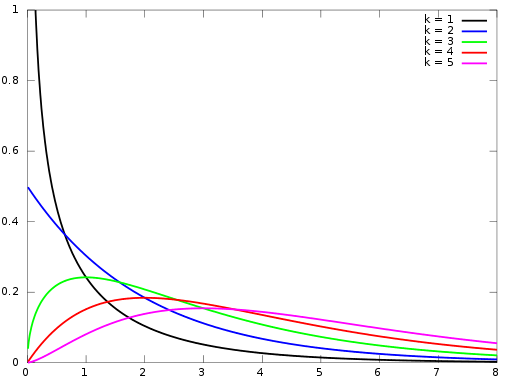
\includegraphics{chisquared.png}}}
		\end{center}
	\end{figure}
	
\end{frame}


\begin{frame}
	\frametitle{Chi-squared test}
	\begin{block}{Intuition}
		Can be thought of as a way to measure the discrepancy between
		\begin{itemize}
			\item the theoretical distribution, and
			\item the observed distribution.
		\end{itemize}
	The greater the discrepancy, the larger the test statistic is: less likely to happen by chance. \textcolor{red}{can explain a bit better the side of the test, and p-val}
	\end{block}
\end{frame}


% another way to forumulate 

%\begin{frame}
%	\begin{block}{Alternative formulation of the Chi-squared test for a $2 \times 2$ table}
%		
%		\begin{itemize}
%			\item A quicker formula for calculating the \hl{test statistic} on
%			a $2 \times 2$ table is
%			\begin{equation}
%				\chi^2 = \frac{n \times (d_1 \cdot h_0 - d_0 \cdot h_1)^2}{d \cdot h
%					\cdot n_1 \cdot n_0}, \quad \mathrm{d.f.} = 1,\nonumber
%			\end{equation}
%			using the previous notation for a $2 \times 2$ table
%		\end{itemize}
%	\end{block}
%\end{frame}




%\begin{frame}
%	\begin{block}{Example 17.1 in Kirkwood \& Sterne}
%		In the example of the \hl{influenza vaccination trial}, the
%		chi-squared is
%		\begin{equation*}
%			\chi^2 = \frac{460 \cdot (20 \cdot 140 - 80 \cdot 220)^2}{100 \cdot 360 \cdot 240 \cdot 220} = 53.01,
%		\end{equation*}
%		which, apart from rounding error, is the same as the value obtained
%		using the formula of observed and expected numbers
%	\end{block}
%\end{frame}






% ---- fisher's exact test -----

\begin{frame}
	\frametitle{(Fisher's) Exact test for $2 \times 2$ tables}
	\begin{block}{}
		When the numbers in the $2 \times 2$ table are\textbf{ very small}, we
		need an \hl{exact test} to compare two proportions \textcolor{red}{why, what happens if insist on chisq}
		
		\begin{itemize}
			\item  Rule of thumb: overall total less than 20, or smallest expected number is less than 5 when total is between 20 to 40.
			\item This is based on calculating the \hl{exact probabilities} of
			the \textbf{observed table} and of \textbf{more extreme tables }with the same row and
			column totals, using the following formula:
			\begin{equation}
				\text{Exact probability} = \frac{d! \cdot h! \cdot n_1! \cdot n_0!}{n! \cdot d_1! \cdot d_0! \cdot h_1! \cdot h_0!},\nonumber
			\end{equation}
			with the standard notation for a $2 \times 2$ table
		\end{itemize}
	\end{block}
\end{frame}



\begin{frame}
	\frametitle{(Fisher's) Exact test for $2 \times 2$ tables}
	\frametitle{}
	\begin{block}{P-values in exact test for $2 \times 2$ tables}
		\begin{itemize}
			\item There are \emph{two} approaches to calculate the (two-sided) $P$-value:
			\begin{itemize}
				\vspace*{1em}   
				\item $\text{$P$-value (approach $\mathrm{I}$)} = \text{probability of
					observed table}$ $ + \text{probability of less probable tables}$
				
				\vspace*{1em}    
				\item $\text{$P$-value (approach $\mathrm{II}$)} = 2 \cdot
				(\text{probability of observed table} $ $ + \text{probability of more extreme tables in the same direction)}$
			\end{itemize}
		\end{itemize}
	\end{block}
\end{frame}



% ---- example 17.2 ----

\begin{frame}
\frametitle{Example: 17.2 in Kirkwood \& Sterne}
\begin{block}{}
  Consider the results from a study to compare two treatment regimes
  for \hl{controlling bleeding} in haemophiliacs ('\emph{bl?dere}')
  undergoing surgery
\begin{table}
\begin{normalsize}
\begin{tabular}{lccc}
\hline
& \multicolumn{2}{c}{\textbf{Bleeding complications}} &
\\
\cline{2-3}
\textbf{Treatment regime} & \textbf{Yes} & \textbf{No} & \textbf{Total}
\\
\hline
\textbf{A (group 1)} & 1 ($d_1$) & 12 ($h_1$) & 13 ($n_1$)
\\
\textbf{B (group 0)} & 3 ($d_0$) & 9 ($h_0$) & 12 ($n_0$)
\\
\hline
\textbf{Total} & 4 ($d$) & 21 ($h$) & 25 ($n$)
\\
\hline
\end{tabular}
\end{normalsize}
\end{table}
Only one (8\%) of the 13 haemophiliacs given treatment regime A suffered bleeding complications, compared to three (25\%) of the 12 given regime B
\end{block}
\end{frame}

\begin{frame}
\begin{block}{}
These numbers are too small for the \hl{chi-squared test} to be valid:
\begin{itemize}
\item{the overall total, 25, is less than 40, and}
\item{the smallest expected value, $4/25 \cdot 12=1.9$ (complications with regime B), is less than 5}
\end{itemize}

\vspace*{1em}
The \hl{exact test} should therefore be used
\end{block}
\end{frame}

\begin{frame}
\begin{block}{}
The \hl{exact probability} of the observed table is
\begin{eqnarray*}
\text{Exact probability} & = & \frac{4! \cdot 21! \cdot 13! \cdot 12!}{25! \cdot 1! \cdot 3! \cdot 12! \cdot 9!}
\\
& = & 0.2261
\end{eqnarray*}
In addition, we need to calculate the probability that a \hl{more
  extreme table} (with the same row and column totals as the observed
table) could occur by chance \textit{under the null hypothesis} that there is
no difference between the two treatment regimes
\end{block}
\end{frame}

\begin{frame}
\begin{block}{}
\begin{table}
\begin{footnotesize}
\begin{tabular}{cc}
\begin{tabular}{lccc}
& & & \textbf{Total}
\\
\hline
& \textcolor{blue}{0} &  \textcolor{blue}{13} & 13 \\
&  \textcolor{blue}{4} &  \textcolor{blue}{8} & 12 \\
\textbf{Total} & 4 & 21& 25 \\
\hline
& & $P$=0.0391 &
\end{tabular}
&
\begin{tabular}{lccc}
& & & \textbf{Total}
\\
\hline
& 1 & 12 & 13 \\
& 3 & 9 & 12 \\
\textbf{Total} & 4 & 21& 25 \\
\hline
& & $P$=0.2261 &
\end{tabular}
\\ \\ \\ \\
\begin{tabular}{lccc}
& & & \textbf{Total}
\\
\hline
&  \textcolor{blue}{2} &  \textcolor{blue}{11} & 13 \\
&  \textcolor{blue}{2} &  \textcolor{blue}{10} & 12 \\
\textbf{Total} & 4 & 21& 25 \\
\hline
& & $P$=0.4070 &
\end{tabular}
&
\begin{tabular}{lccc}
& & & \textbf{Total}
\\
\hline
&  \textcolor{blue}{3} &  \textcolor{blue}{10} & 13 \\
&  \textcolor{blue}{1} &  \textcolor{blue}{11} & 12 \\
\textbf{Total} & 4 & 21& 25 \\
\hline
& & $P$=0.2713 &
\end{tabular}
\\ \\ \\ \\
\begin{tabular}{lccc}
& & & \textbf{Total}
\\
\hline
&  \textcolor{blue}{4} &  \textcolor{blue}{9} & 13 \\
&  \textcolor{blue}{0} &  \textcolor{blue}{12} & 12 \\
\textbf{Total} & 4 & 21& 25 \\
\hline
& & $P$=0.0565 &
\end{tabular}
\end{tabular}
\end{footnotesize}
\end{table}
\end{block}
\end{frame}

\begin{frame}
\begin{block}{}
According to \hl{approach $\mathrm{I}$} the total probability needed for the (two-sided) \hl{$P$-value} is:
\begin{equation*}
0.2261 + 0.0565 + 0.0391 = 0.3217,
\end{equation*}
and so there is \textbf{no evidence against the null hypothesis }of no difference between the regimes. 

\vspace*{2em}
According to \hl{approach $\mathrm{II}$} the (two-sided) \hl{$P$-value} obtained is:
\begin{equation*}
2 \cdot (0.2261 + 0.0391) = 0.5304.
\end{equation*}

\vspace*{2em}
The two approaches lead to different p-values for small cell counts! For increasing $n$ they will become more similar.

\textcolor{red}{explain why, and in detail }
\end{block}
\end{frame}

% ------- test validity ------- 

\begin{frame}
	\begin{block}{Test validity}
		\begin{itemize}
			\item The \hl{chi-squared test} is valid when:
			\begin{itemize}
				\item{The overall total is more than 40, regardless of the expected
					values, or}
				\item{The overall total is between 20 and 40 provided all the expected
					values are at least 5}
			\end{itemize}
			\item The use of the \hl{exact test} is recommended when:
			\begin{itemize}
				\item{The overall total of the table is less than 20, or}
				\item{The overall total is between 20 and 40 and the smallest of the
					four expected numbers is less than 5}
			\end{itemize}
		\end{itemize}
	\end{block}
\end{frame}



\begin{frame}
	\begin{block}{Important}
		\begin{itemize}
			\item The chi-squared test produce \hl{only a p-value}
			\item Often a meassure of the effect with confidence intervals are
			required when publishing (for instance odds ratio, relative risk or
			the risk difference)
		\end{itemize}
	\end{block}
\end{frame}


% -------- larger tables --------
\begin{frame}
	\frametitle{Chi-squared test for $r \times c$ tables}
	\begin{block}{}
		The \hl{chi-squared test} can also be applied to larger
		tables, generally called \hl{$r \times c$ tables}, where $r$
		denotes the number of rows in the table and $c$ the number of
		columns
		
		\vspace{0.2cm}
		The \hl{test statistic} is:
		\begin{equation}
			\chi^2 = \sum_i \frac{(O_i - E_i)^2}{E_i}, \quad \mathrm{d.f.} = (r - 1) \cdot (c - 1),
		\end{equation}
		which is chi-squared distributed with $(r - 1) \cdot (c - 1)$ degrees
		of freedom under the null hypothesis
		
		\vspace{0.2cm}
		The general rule for calculating an \hl{expected number} is:
		\begin{equation}
			E = \frac{\text{column total} \cdot \text{row total}}{\text{overall total}}
		\end{equation}

	\end{block}
\end{frame}



\begin{frame}
	\frametitle{Chi-squared test for $r \times c$ tables}
	\textbf{Test validity}
	The approximation of the chi-squared test is valid when:
	\begin{itemize}
		\item{less than 20\% of the expected numbers are under 5, and}
		\item{none of the expected numbers is less than 1}
	\end{itemize}
	Sometimes this restriction \hl{can be overcome by combining rows
		(or columns)} with low expected numbers, providing that these
	combinations make biological sense

\end{frame}




% ----- example 17.3 ------ 
\begin{frame}
\begin{block}{Example: 17.3 in Kirkwood \& Sterne}
  Consider the results from a survey to compare the \hl{principal
    water sources} in three villages in West Africa. 

The numbers of
  households using a river, a pond, or a spring are given. We will
  treat the \hl{water source} as outcome and \hl{village} as
  exposure, so column precentages are displayed.
\begin{table}
\begin{footnotesize}
\begin{tabular}{lcccc}
Observed numbers & & & &
\\
\hline
& \multicolumn{3}{c}{\textbf{Water source}} &
\\
\cline{2-4}
\textbf{Village} & \textbf{River} & \textbf{Pond} & \textbf{Spring} & \textbf{Total}
\\
\hline
\textbf{A} & 20 (40.0\%) & 18 (36.0\%) & 12 (24.0\%) & 50 (100.0\%)
\\
\textbf{B} & 32 (53.3\%) & 20 (33.3\%) & 8 (13.3\%) & 60 (100.0\%)
\\
\textbf{C} & 18 (45.0\%) & 12 (30.0\%) & 10 (25.0\%) & 40 (100.0\%)
\\
\hline
\textbf{Total} & 70 (46.7\%) & 50 (33.3\%) & 30 (20.0\%) & 150 (100.0\%)
\\
\hline
\end{tabular}
\end{footnotesize}
\end{table}
\end{block}
\end{frame}

\begin{frame}
\begin{block}{}
  Overall, 70 of the 150 households use a river. If there were no
  difference between villages, one would expect this same proportion
  of river usage in each village. Thus the \hl{expected numbers} of
  households using a river in villages A, B and C, respectively, are:
\begin{equation*}
\frac{70}{150} \cdot 50 = 23.3, \quad \frac{70}{150} \cdot 60 = 28.0 \quad \text{and} \quad \frac{70}{150} \cdot 40 = 18.7.
\end{equation*}
We use the same procedure to calculate the expected numbers of
households using a pond and a spring in the villages.
\begin{table}
\begin{tiny}
\begin{tabular}{lcccc}
Expected numbers & & & &
\\
\hline
& \multicolumn{3}{c}{\textbf{Water source}} &
\\
\cline{2-4}
\textbf{Village} & \textbf{River} & \textbf{Pond} & \textbf{Spring} & \textbf{Total}
\\
\hline
\textbf{A} & 23.3 & 16.7 & 10.0 & 50
\\
\textbf{B} & 28.0 & 20.0 & 12.0 & 60
\\
\textbf{C} & 18.7 & 13.3 & 8.0 & 40
\\
\hline
\textbf{Total} & 70 & 50 & 30 & 150
\\
\hline
\end{tabular}
\end{tiny}
\end{table}
\end{block}
\end{frame}

\begin{frame}
\begin{block}{}
The observed value of the \hl{test statistic} is:
\begin{eqnarray*}
\chi^2 & = & \frac{(20 - 23.3)^2}{23.3} + \frac{(18 - 16.7)^2}{16.7} + \frac{(12 - 10.0)^2}{10.0} \\
& & \quad + \frac{(32 - 28.0)^2}{28.0} + \frac{(18 - 18.7)^2}{18.7} + \frac{(20 - 20.0)^2}{20.0}  \\
& & \quad + \frac{(8 - 12.0)^2}{12.0} + \frac{(12 - 13.3)^2}{13.3} + \frac{(10 - 8.0)^2}{8.0} \\
& = & 3.53,
\end{eqnarray*}
with $\mathrm{d.f.}=(r - 1) \cdot (c - 1) = 2 \cdot 2 = 4$ degrees of freedom.
\end{block}

\begin{block}{}
  The corresponding \hl{$\bm{P}$-value} is
  0.47. This means that there is no evidence of a difference between
  the villages in the proportion of households using different water
  sources.
\end{block}

\end{frame}



\frame{ 
\frametitle{Final Remark (1): McNemars test}
  \begin{block}{}
    \begin{itemize}
    \item A special case of the 2x2 table for \hl{paired categorical
        data}
    \item For example when measuring the presence/absence of something at
      two time points for each individual
      \vspace*{2em}
    \item In the menu: \emph{'Statistics -> Epidemiology and related -> Tables for Epidemiologists -> Matched case-control Calculator'}\\
    or directly use the command \texttt{mcci}
    \end{itemize}
  \end{block}
}

\frame{ 
\frametitle{Final Remark (2): Chi squared versus Fisher's exact test}
  \begin{block}{}
    \begin{itemize}
    \item If the exact test works for both small and large samples, it is \hl{natural to ask if we shall always use the exact test}.
    \item The two tests \hl{have different assumptions}
    \item The \hl{exact test can be (very) conservative}; giving to high p-values and low power
    \end{itemize}
    
    \footnotesize \center Read more in e.g. Lydersen, Fagerland, Laake, \emph{Recommended tests for association in 2x2 tables}, Statistics in Medicine, 2009: Fisher's exact should never be used without the mid-P correction \normalsize
    
  \end{block}
}










% --------- STATA examples --------

\begin{frame}[fragile]{Table analysis in STATA}
	\begin{block}{Aggregated data (Example KS 17.1)}
		
		With menus: \emph{'Statistics -> Epidemiology and related -> Tables for Epidemiologists -> Cohort study risk  ratio etc. Calculator'}
			\begin{itemize}
			
			\item Fill in number of exposed cases 20, non-exposed cases 80, exposed non-cases 220 and non-exposed non-case 140,
			
			\item Press \emph{'OK'}.
		\end{itemize}
		
	\end{block}
	
\end{frame}



\begin{frame}
	\frametitle{Table analysis in STATA}
	\begin{block}{Aggregated data (Example KS 17.1)}
			\begin{figure}[H]
			\begin{center}
				{\scalebox{0.5}{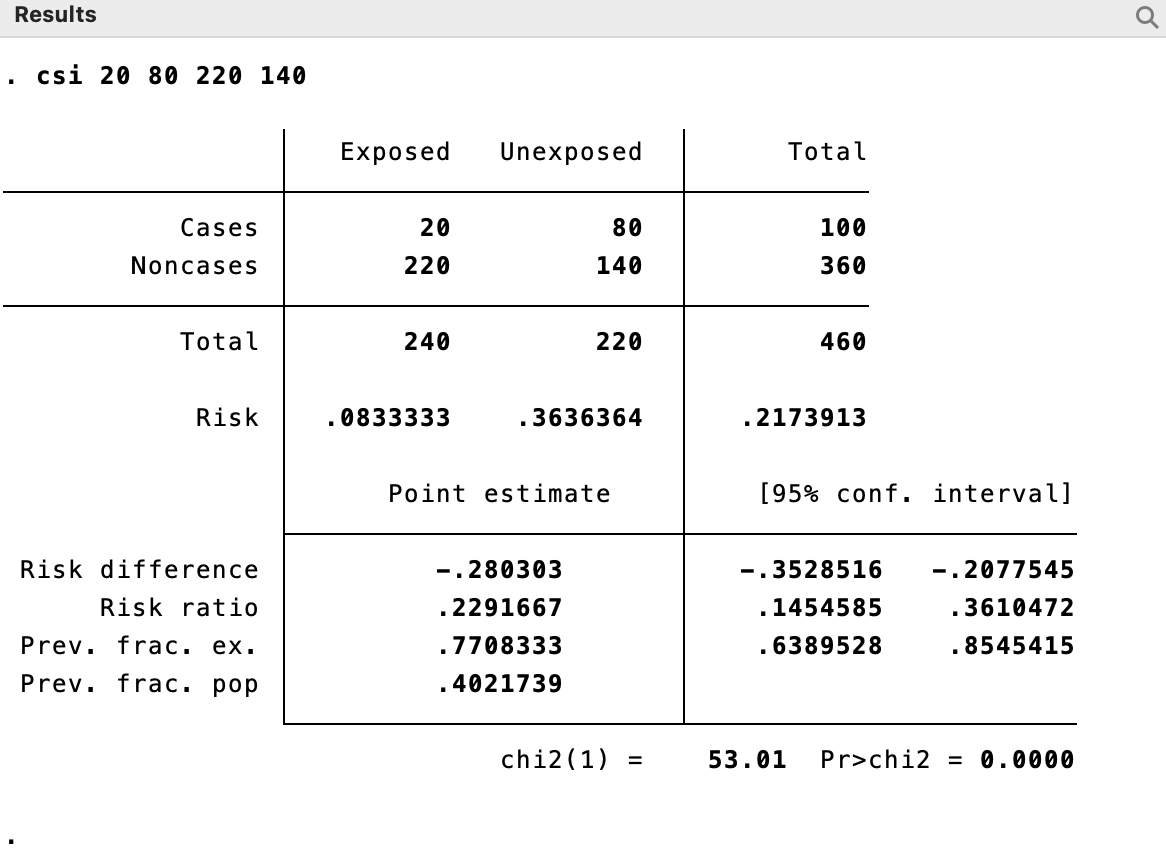
\includegraphics{stata_ks171.png}}}
			\end{center}
		\end{figure}
	\end{block}
	
\end{frame}

%\begin{frame}[fragile]{Output}
%	\scriptsize
%	\begin{verbatim}
	%. csi 20 80 220 140
	%
	%                 |   Exposed   Unexposed  |      Total
	%-----------------+------------------------+------------
	%           Cases |        20          80  |        100
	%        Noncases |       220         140  |        360
	%-----------------+------------------------+------------
	%           Total |       240         220  |        460
	%                 |                        |
	%            Risk |  .0833333    .3636364  |   .2173913
	%                 |                        |
	%                 |      Point estimate    |    [95% Conf. Interval]
	%                |------------------------+------------------------
	% Risk difference |         -.280303       |   -.3528516   -.2077545 
	%      Risk ratio |         .2291667       |    .1454585    .3610472 
	% Prev. frac. ex. |         .7708333       |    .6389528    .8545415 
	% Prev. frac. pop |         .4021739       |
	%                 +-------------------------------------------------
	%                              chi2(1) =    53.01  Pr>chi2 = 0.0000
	
	%	\end{verbatim}
%\normalsize
%\end{frame}
%--- Next Frame ---%
%--- Next Frame ---%

\begin{frame}{More on the STATA-output}
	We see that STATA offers more output than just the  p-value:  
	\begin{itemize}
		\item Risk ratio (relative risk) and risk difference with confidence intervals,  
		\item Odds Ratio with confidence interval
		
		\item Dependent on whether the  exposure is protective or harmful, STATA also  reports:\\
		(if harmful)	
		\begin{itemize}
			\item Attributable  fractions for the exposed, 
			\begin{itemize}
				\item The proportion  of exposed cases that  are  due to the exposure,
			\end{itemize}
			\item Attributable fractions for the total population, 
			\begin{itemize}
				\item The proportion  of cases in  the  population due to the exposure,
			\end{itemize}
		\end{itemize}
		(if protective, our case here)
		\begin{itemize}
			\item Prevented fractions for the exposed, \begin{itemize}
				\item The proportion  of exposed noncases that  are  due to the exposure
			\end{itemize}
			\item Prevented fractions for the total population,
			\begin{itemize}
				\item The proportion  of non-cases in  the  population due to the exposure,
			\end{itemize}
			
		\end{itemize}
	\end{itemize}
\end{frame}



\begin{frame}[fragile]{Table analysis in STATA}
	\begin{block}{Individual data (birth data)}
	
	Want to test the hypothesis $H_0:$ the risk of being a smoker is the same for mothers older than 25 and mothers younger than 25. 
	
	\vspace{0.2cm}
	
	Open data file 
	
	\begin{verbatim}
		use "path_to_your_data_folder/statafiles/birth.dta"
		browse
	\end{verbatim}


	\end{block}
\end{frame}

\begin{frame}[fragile]{Table analysis in STATA}
		\begin{figure}[H]
	\begin{center}
		{\scalebox{0.3}{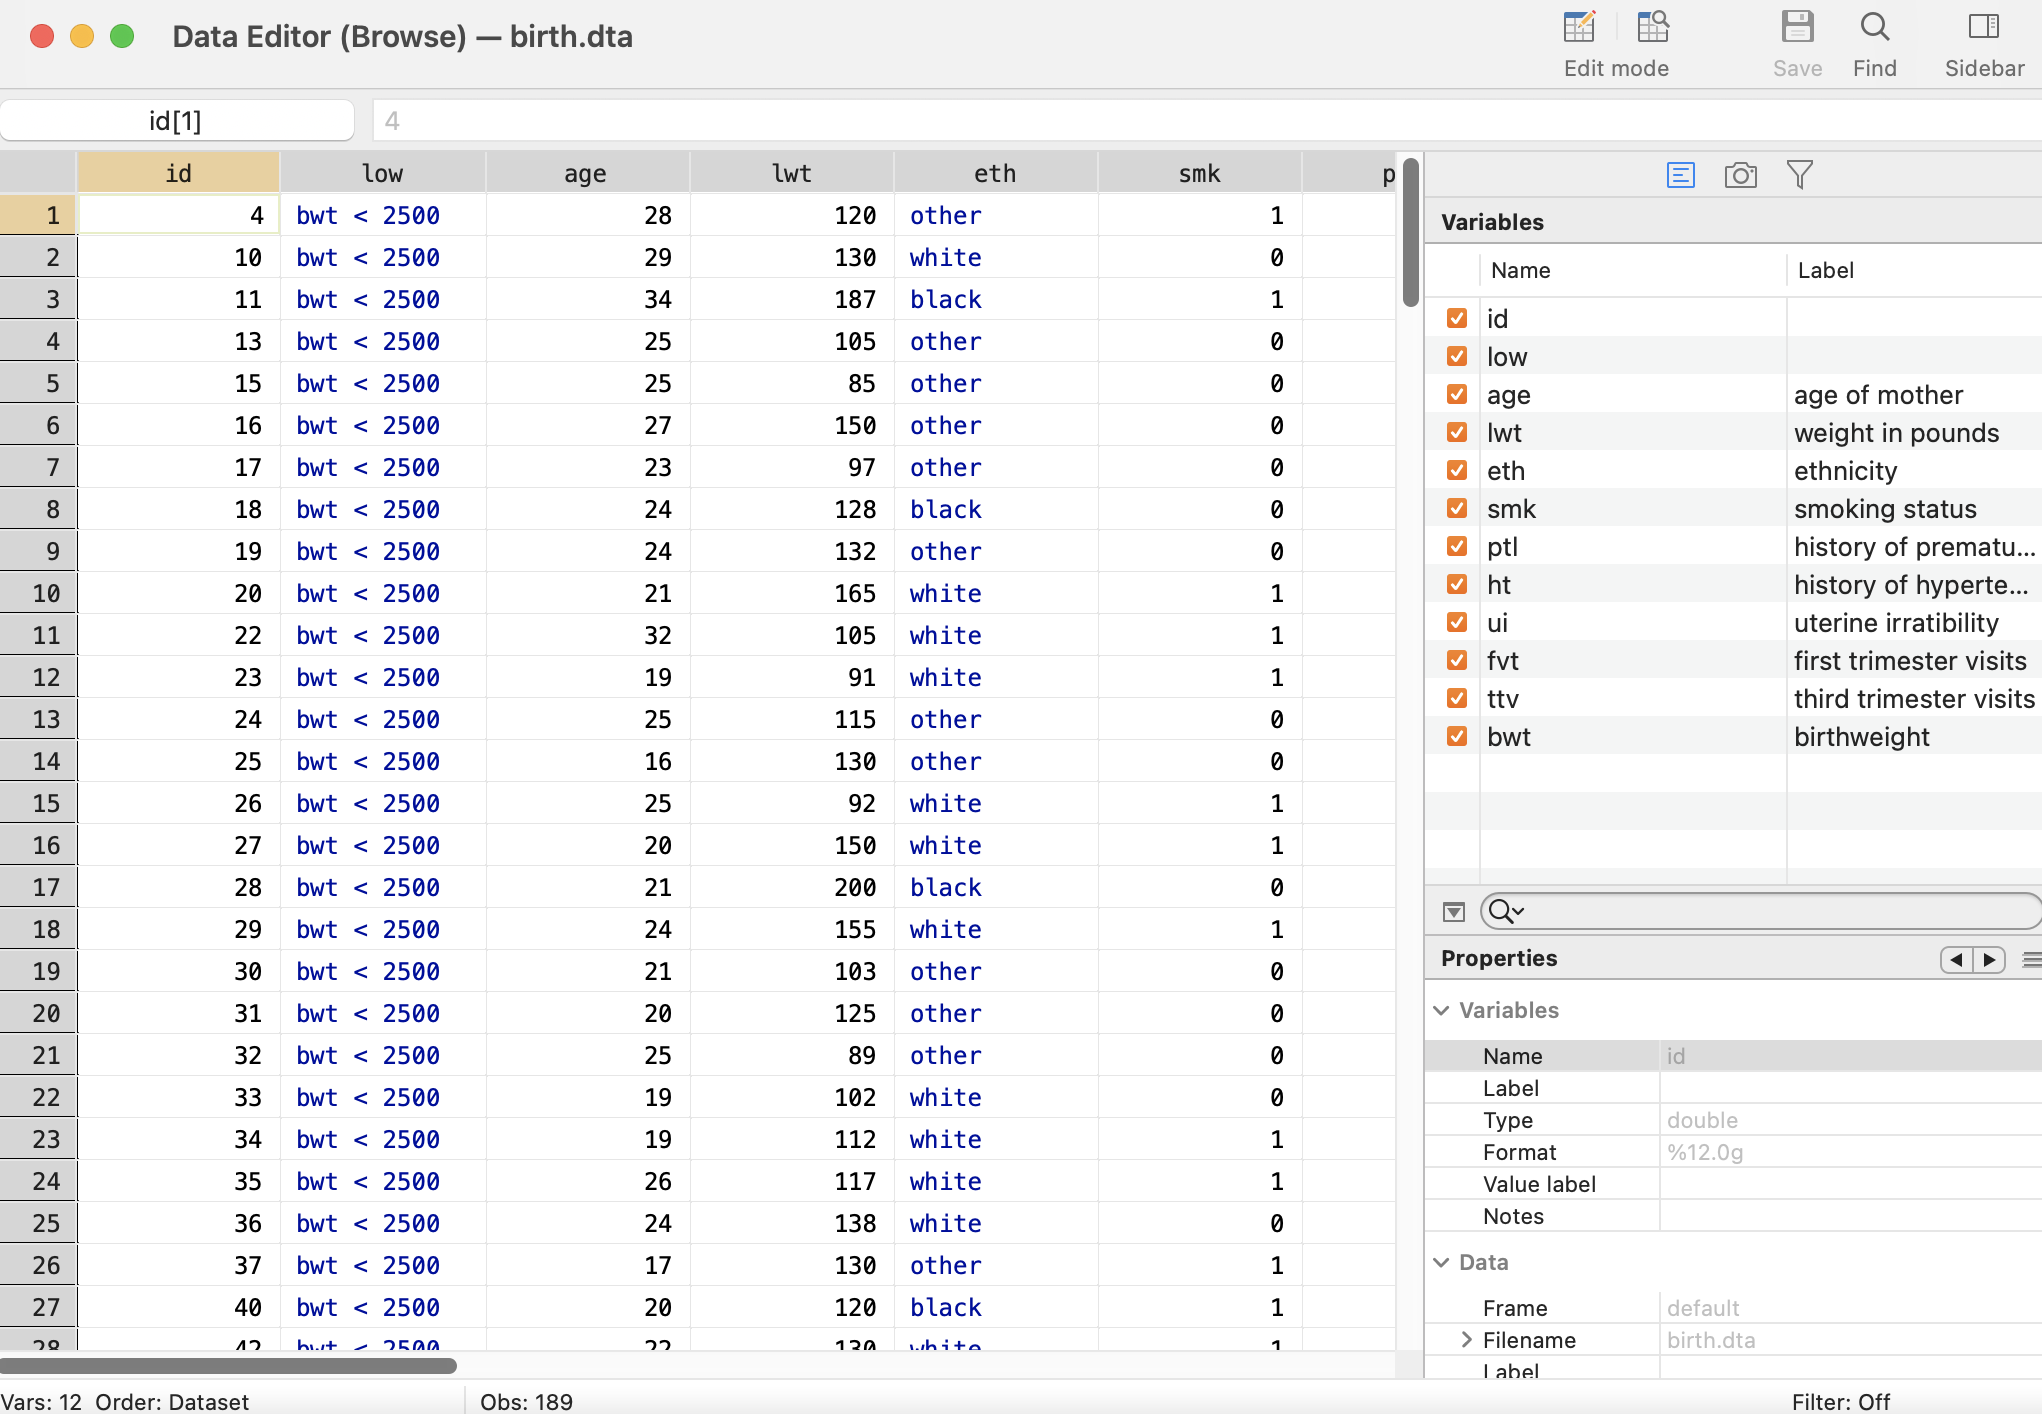
\includegraphics{stata_birthdta.png}}}
	\end{center}
\end{figure}
\end{frame}


\begin{frame}[fragile]{Table analysis in STATA}
	\begin{block}{Individual data (birth data)}
		
		Generate a variable that encodes age < 25 or not: 
		\begin{verbatim}
			gen youngMother = age <25
		\end{verbatim} 
		
		Then carry out analysis between \textbf{smoking} and \textbf{young mother} variables, 
		\vspace{0.2cm}
		Either  use menu: \emph{'Statistics -> Epidemiology and related -> Tables for Epidemiologists -> Cohort study risk  ratio etc. '}, or use commands
		\begin{verbatim}
			cs smk youngMother
		\end{verbatim}  
		or \begin{verbatim}
			tab  smk youngMother, chi2
		\end{verbatim}
		
	\end{block}
\end{frame}





\begin{frame}[fragile]{Table analysis in STATA}
	\begin{block}{Individual data (birth data): risk ratio}
		
		\begin{figure}[H]
			\begin{center}
				{\scalebox{0.5}{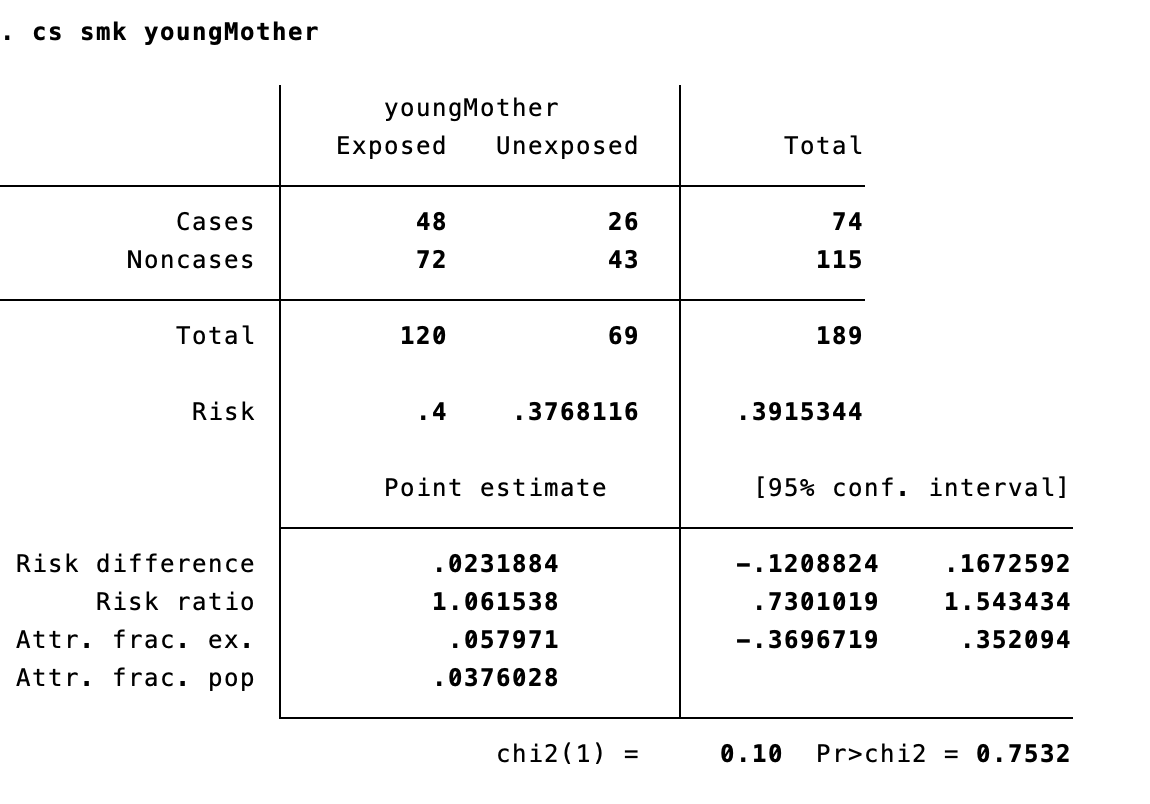
\includegraphics{stata_birth_rr.png}}}
			\end{center}
		\end{figure}
		
		
	\end{block}
\end{frame}

\begin{frame}[fragile]{Table analysis in STATA}
\begin{block}{Individual data (birth data): chi-squared}
	
	\begin{figure}[H]
		\begin{center}
			{\scalebox{0.5}{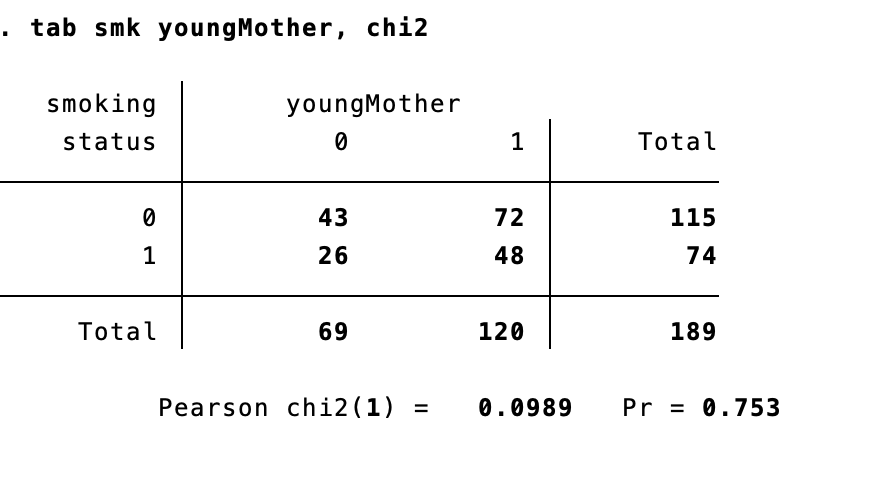
\includegraphics{stata_birth_chi2.png}}}
		\end{center}
	\end{figure}
	
\end{block}
\end{frame}
%\begin{frame}[fragile]{Output}
%	\scriptsize
%	\begin{verbatim}
	% cs smk youngMother 
	%
	%                 | youngMother            |
	%                 |   Exposed   Unexposed  |      Total
	%-----------------+------------------------+------------
	%           Cases |        48          26  |         74
	%        Noncases |        72          43  |        115
	%-----------------+------------------------+------------
	%           Total |       120          69  |        189
	%                 |                        |
	%            Risk |        .4    .3768116  |   .3915344
	%                 |                        |
	%                 |      Point estimate    |    [95% Conf. Interval]
	%                 |------------------------+------------------------
	% Risk difference |         .0231884       |   -.1208824    .1672592 
	%      Risk ratio |         1.061538       |    .7301019    1.543434 
	%Attr. frac. ex. |          .057971       |   -.3696719     .352094 
	%Attr. frac. pop |         .0376028       |
	%                 +-------------------------------------------------
	%                              chi2(1) =     0.10  Pr>chi2 = 0.7532		
	%	\end{verbatim}
%	\normalsize
%\end{frame}




%\begin{frame}[fragile]{Output}
%	\scriptsize
%	\begin{verbatim}
	%. tab smk youngMother, chi2  expected 
	%
	%+--------------------+
	%| Key                |
	%|--------------------|
	%|     frequency      |
	%| expected frequency |
	%+--------------------+
	%
	%   smoking |      youngMother
	%    status |         0          1 |     Total
	%-----------+----------------------+----------
	%         0 |        43         72 |       115 
	%           |      42.0       73.0 |     115.0 
	%-----------+----------------------+----------
	%        1 |        26         48 |        74 
	%          |      27.0       47.0 |      74.0 
	%-----------+----------------------+----------
	%     Total |        69        120 |       189 
	%           |      69.0      120.0 |     189.0 
	%
	%          Pearson chi2(1) =   0.0989   Pr = 0.753
	%
	%. 
	%		
	%	\end{verbatim}
%	\normalsize
%\end{frame}
%--- Next Frame ---%
%--- Next Frame ---%
%--- Next Frame ---%




\begin{frame}
	\frametitle{Table analysis in STATA}
	
	\begin{block}{Exact test (example KS 17.2)}
		\begin{itemize}
		\item Use the menu (as we did for Example 17.1 before): \emph{'Statistics -> Epidemiology and related -> Tables for Epidemiologists -> Cohort study risk  ratio etc. Calculator'}
		\item Fill in  number of exposed cases, non-exposed cases, exposed non-cases and non-exposed non-case (we consider treatment regime A to be exposure)
		\item Select ``Fisher's exact $p$'' in order to compute the correct p-value, and select a confidence level
		\item Press \emph{'OK'}.
	\end{itemize}
	\end{block}

\end{frame}

\begin{frame}[fragile]{Table analysis in STATA}
	\begin{block}{Exact test (example KS 17.2)}
		
		\begin{figure}[H]
			\begin{center}
				{\scalebox{0.5}{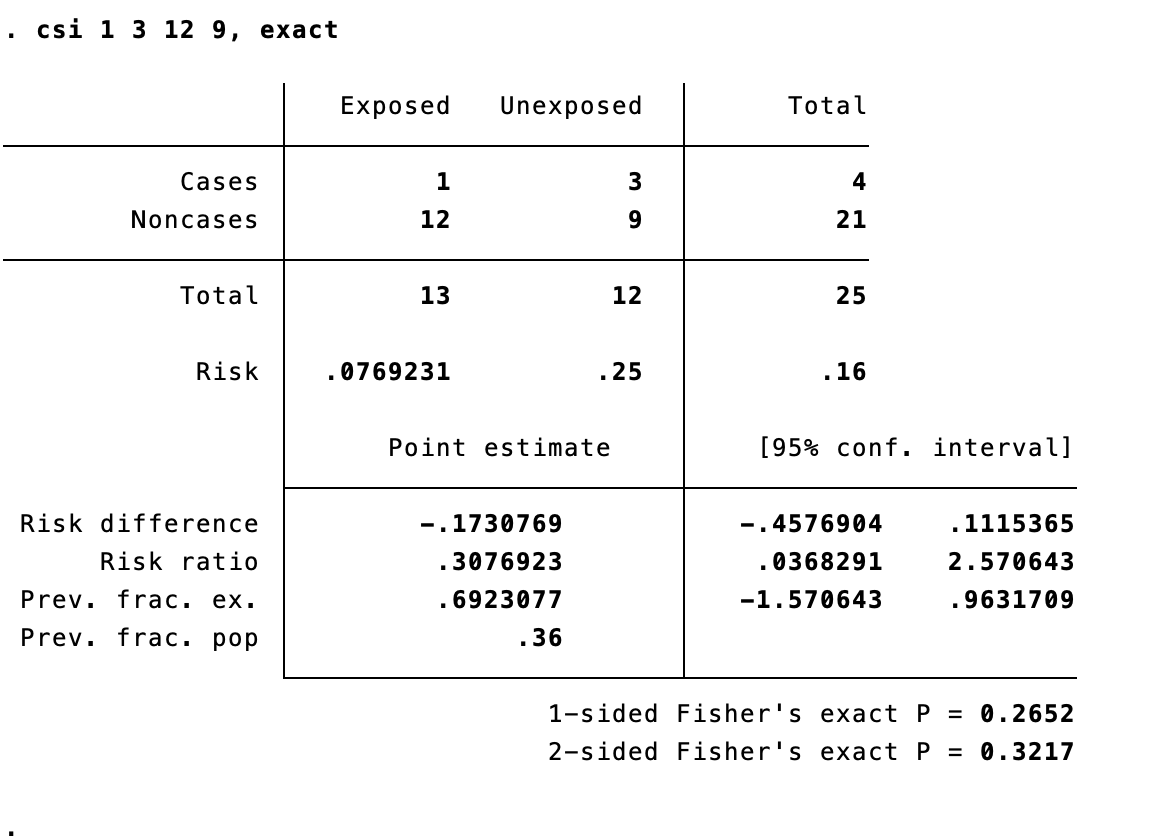
\includegraphics{stata_ks172.png}}}
			\end{center}
		\end{figure}
		
	\end{block}
\end{frame}

%\begin{frame}[fragile]{Output}
%\scriptsize
%\begin{verbatim}
%. csi 1 3 12 9, or exact
%                 |   Exposed   Unexposed  |      Total
%-----------------+------------------------+------------
%           Cases |         1           3  |          4
%        Noncases |        12           9  |         21
%-----------------+------------------------+------------
%           Total |        13          12  |         25
%                 |                        |
%            Risk |  .0769231         .25  |        .16
%                 |                        |
%                 |      Point estimate    |    [95% Conf. Interval]
%                 |------------------------+------------------------
% Risk difference |        -.1730769       |   -.4576904    .1115365 
%      Risk ratio |         .3076923       |    .0368291    2.570643 
% Prev. frac. ex. |         .6923077       |   -1.570643    .9631709 
% Prev. frac. pop |              .36       |
%      Odds ratio |              .25       |           0    2.156895 (Cornfield)
%                 +-------------------------------------------------
%                                  1-sided Fisher's exact P = 0.2652
%                                  2-sided Fisher's exact P = 0.3217
%
%\end{verbatim}
%\normalsize    
%\end{frame}



\begin{frame}[fragile]{Table analysis in STATA}
	\begin{block}{Larger contingency tables}
			\begin{itemize}
			\item Either menu: \emph{'Statistics -> Summaries, tables and tests -> Frequency tables -> Table calculator},
			\item Fill in count data 'row-wise' separated by\textbackslash, 
			\item Click $\chi^2$ (and expected)
		\end{itemize}
		or by command
		\begin{verbatim}
			tabi 20 18 12 \ 32 20 8 \ 18 12 10, chi2 expected
		\end{verbatim}
	\end{block}

\end{frame}


\begin{frame}[fragile]{Table analysis in STATA}
	\begin{block}{Larger contingency tables}
		
		\begin{figure}[H]
			\begin{center}
				{\scalebox{0.4}{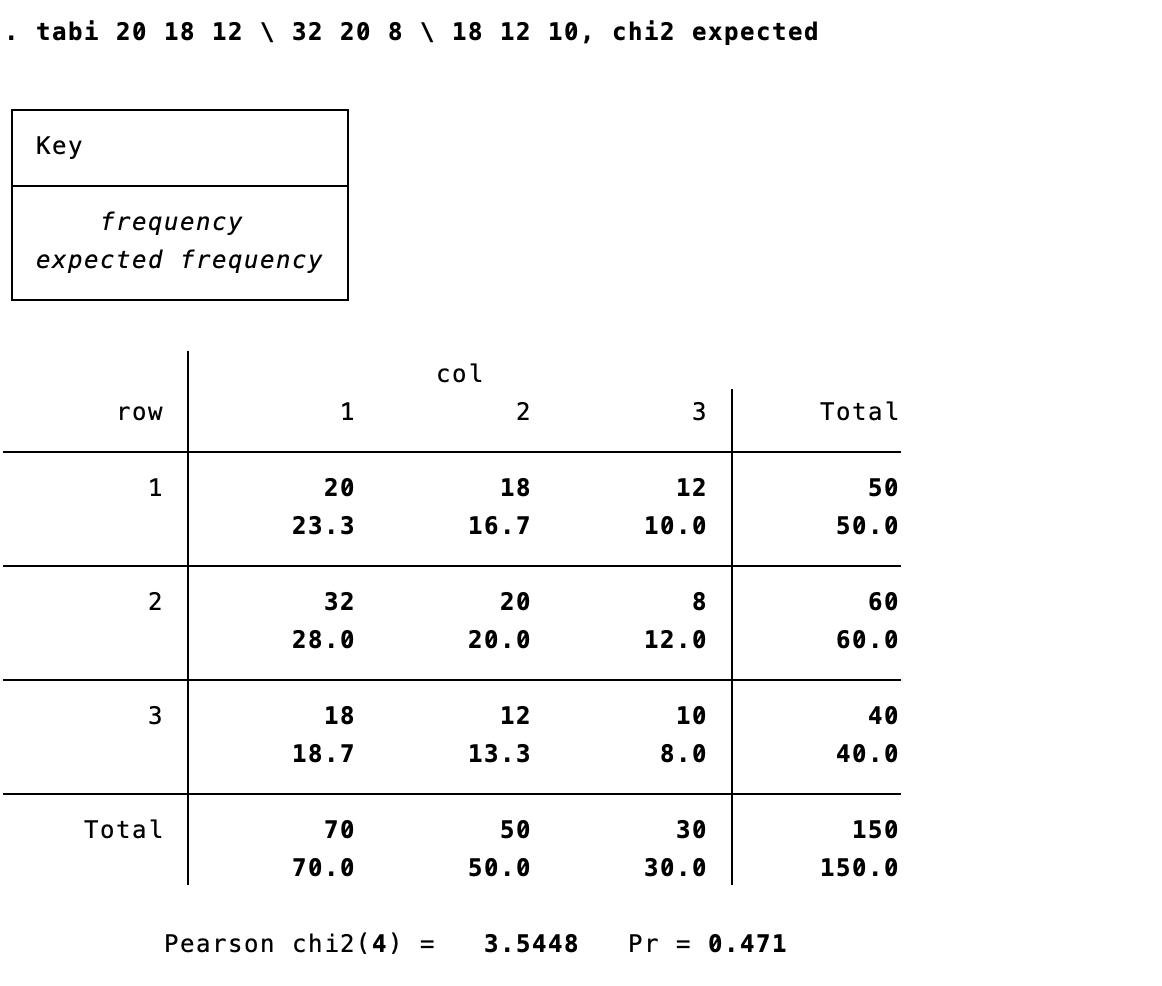
\includegraphics{stata_chi2_3by2.png}}}
			\end{center}
		\end{figure}
		
	\end{block}
\end{frame}

%--- Next Frame ---%
%\begin{frame}[fragile]{Output}
%	\tiny
%	\begin{verbatim}
	%		. tabi 20 18 12 \ 32 20 8 \ 18 12 10, chi2 expected
	%
	%		+--------------------+
	%		| Key                |
	%		|--------------------|
	%		|     frequency      |
	%		| expected frequency |
	%		+--------------------+
	%
	%		           |               col
	%		       row |         1          2          3 |     Total
	%		-----------+---------------------------------+----------
	%		         1 |        20         18         12 |        50 
	%		           |      23.3       16.7       10.0 |      50.0 
	%		-----------+---------------------------------+----------
	%		         2 |        32         20          8 |        60 
	%		           |      28.0       20.0       12.0 |      60.0 
	%		-----------+---------------------------------+----------
	%		         3 |        18         12         10 |        40 
	%		           |      18.7       13.3        8.0 |      40.0 
	%		-----------+---------------------------------+----------
	%		     Total |        70         50         30 |       150 
	%		           |      70.0       50.0       30.0 |     150.0 
	%
	%		          Pearson chi2(4) =   3.5448   Pr = 0.471
	%	\end{verbatim}
%	\normalsize
%\end{frame}


\section{Summary}

\frame{ 
\frametitle{Summary}
  \begin{block}{Key words}
    \begin{itemize}
    \item Contigency tables
    \item Chi-squared tests for $2 \times 2$ and $r \times c$ tables 
    \item Exact tests
    \end{itemize}
  \end{block}
  \begin{block}{Notation}
    \begin{itemize}
    \item $\chi_n^2$
    \item $O_i$ and $E_i$
    \item $n, d, h$
    \end{itemize}
  \end{block}
}

\end{document}

